Die Software PRTG\(\footnote{Früher Pässler Router Traffic Grapher}\)
der deutschen Firma Paessler GmbH bietet eine Vielzahl an Tools um
nahezu jede Komponente eines Netzwerks zu überwachen. Einige wichtige
Features bilden:

\begin{itemize}
\item
  Unterstützung aller gängige Agents: SNMP, WMI, SSH bzw. Agentless:
  SQL, Ping, REST APIs und viel mehr.
\item
  Maps und Dashboard: Intuitive Erstellung von Dashboards zur echtzeit
  Überwachung mit Live-Stausinformationen
\item
  Flexibler Alarm: PRTG alarmiert automatisch den Administrator, sobald
  Problem oder Anomalien entdeckt werden.
\end{itemize}

Paessler bietet mehrere Lizenzen an, die sich haupsächlich durch die
Anzahl der Sensoren unterscheiden. Angefangen bei 1.300€ mit 500
unterstützen Sensoren für kleine Unternehmen bis hin zu 12.500€ mit
unbegrenzten Sensoren für größere Unternehmen, ist für jeden was dabei.
Zu Testzwecken stellt Paessler jedem eine 30 Tage Testversion zur
Verfügung.

\hypertarget{installation-erste-schritte}{%
\section{Installation \& Erste
Schritte}\label{installation-erste-schritte}}

Die Installation des Tools ist intuitiv und dauert nur wenige Minuten.
Nachdem PRTG heruntergeladen ist, wird die Software installiert und
automatisch gestartet. Es handelt sich hierbei um eine Webapplikation,
die über die IP-Adresse des Computers erreichbar ist und über jeden
Webbrowser erreichbar ist, der den Server erreichen kann.

\begin{figure}[!htb]
\centering
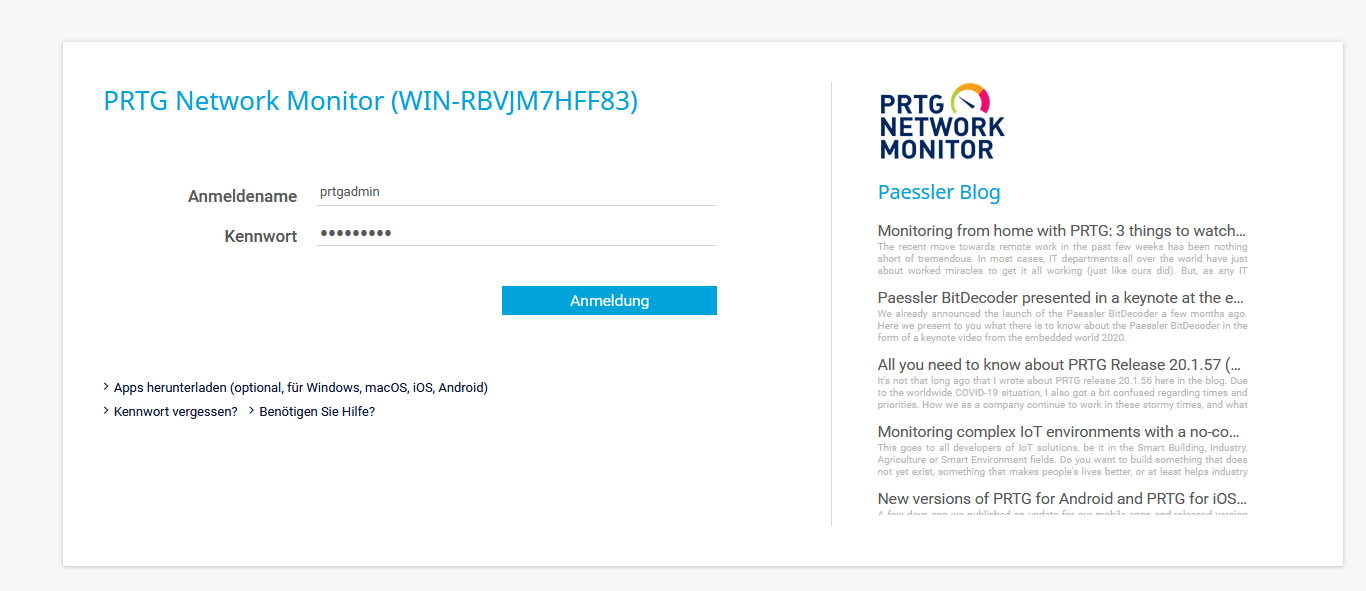
\includegraphics{./images/prtg_welcome.png}
\caption{PRTG Anmeldemaske}\label{prtg-anmeldemaske}
\end{figure}

Bevor man jedoch anfängt mit PRTF zu arbeiten, sollten einem einige
Begriffe geläufig sein. Eineer dieser Begriffe ist der Sensor. Sensoren
sind das um und auf der PRTG Network Monitor Software. Ein Sensor ist
ein Messpunkt, der einen \emph{Aspekt} auf einem Gerät überwacht.
Beispiele dafür wären CPU-Auslastung eines Servers oder die
Portauslastung eines Interfaces auf einem Switch. So ermöglichen eine
Vielzahl von Sensoren die Rundumüberwachung verschiedenster Geräte. Ein
Sensor schleust Daten in einen \emph{Kanal}. So hat der Ping Sensor die
Kanäle Latenz(ms), Paketverlust(\%), etc. .

\hypertarget{lab-uxfcberwachung-von-linux-und-windows-server}{%
\section{LAB: Überwachung von Linux und Windows
Server}\label{lab-uxfcberwachung-von-linux-und-windows-server}}

Das folgende Kapitel beschäftigt sich mit der Überwachung einer
einfachen Serverinfrastruktur.

\hypertarget{topologie}{%
\subsection{Topologie}\label{topologie}}

\begin{figure}[!htb]
\centering
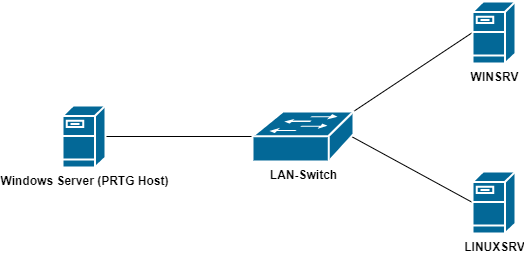
\includegraphics{./images/prtg_architektur.png}
\caption{PRTG LAB Architektur}
\end{figure}

Die Infrastruktur besteht aus drei Servern:

\begin{itemize}
\tightlist
\item
  Windows Server (PRTG Host): Der Monitoring Server
\item
  WINSRV: Windows Server
\item
  LINUXSRV: Linux Server mit einem Apache Server
\end{itemize}

\hypertarget{uxfcberwachung-linux-server}{%
\subsection{Überwachung Linux
Server}\label{uxfcberwachung-linux-server}}

Im ersten Schritt muss das Gerät registriert werden. Dazu im Reiter
\emph{Geräte} auf \emph{Gerät hinzufügen} klciken und einen Gruppe nach
belieben auswählen\$\textbackslash footnote\{Wir haben die Gruppe
\emph{Linux/ macOS / Unix} gewählt\}. Danach erscheint es in der
Geräteliste:

\begin{figure}[!htb]
\centering
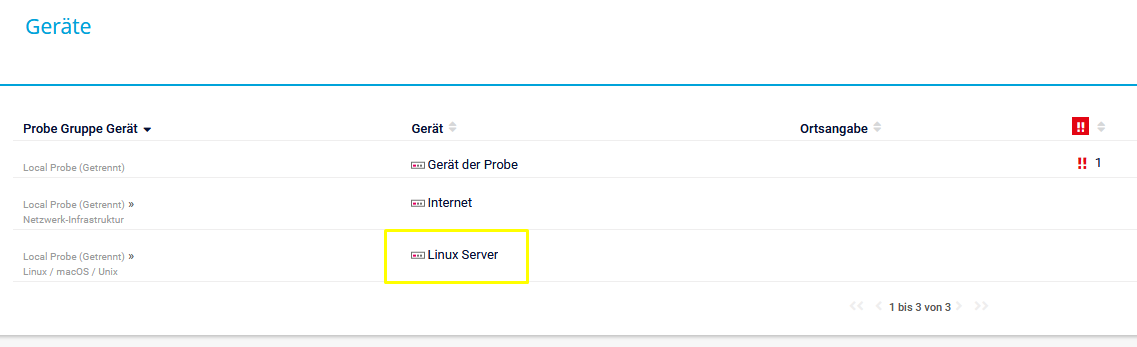
\includegraphics{./images/prtg_linux-server.png}
\caption{PRTG Gerät: Linux Server}
\end{figure}

Die Überwachung eines Linux Servers funktioniert meist Agentless. Es
muss also auf dem Zielgerät nichts installiert werden und
Informationsafrage findet über Protokolle wie SSH, HTTP oder SNMP statt.
Dementsprechend ist die Konfiguration von Sensoren für Linux System
ziemlich straight-forward. Nichtsdestotrotz mussten einige
Vorbereitungen getroffen werden:

\begin{enumerate}
\def\labelenumi{\arabic{enumi}.}
\item
  Open-SSH Server
  installieren\(\footnote{Meist vorinstalliert, bei uns (Linux Mint) jedoch nicht}\)
\item
  Apache Server installieren\(\footnote{apache2}\)
\end{enumerate}

\hypertarget{erster-sensor-ping}{%
\subsubsection{Erster Sensor: Ping}\label{erster-sensor-ping}}

Auf der Geräteseite des Linux Servers kann in der Sensorenbox via Klick
auf das ``+'' ein Sensor hinzugefügt werden.

\begin{figure}[!htb]
\centering
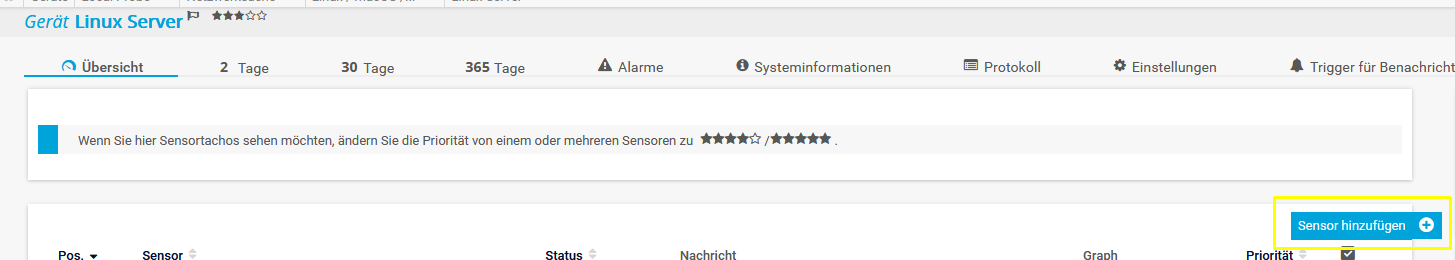
\includegraphics{./images/prtg_add_sensor.png}
\caption{PRTG Sensor hinzufügen}
\end{figure}

Im nächsten Schritt ist der gewünschte Sensortyp auszuwählen, in unserem
Fall Ping. Danach sind einige Paramter einzugeben, wir lassen sie auf
den Defaulteinstellungen. Nach einer kurzen Wartezeit, kann man sich mit
Klick auf den Ping Sensor eine Statistik über die abgesetzten Pings
anschauen.

\begin{figure}[!htb]
\centering
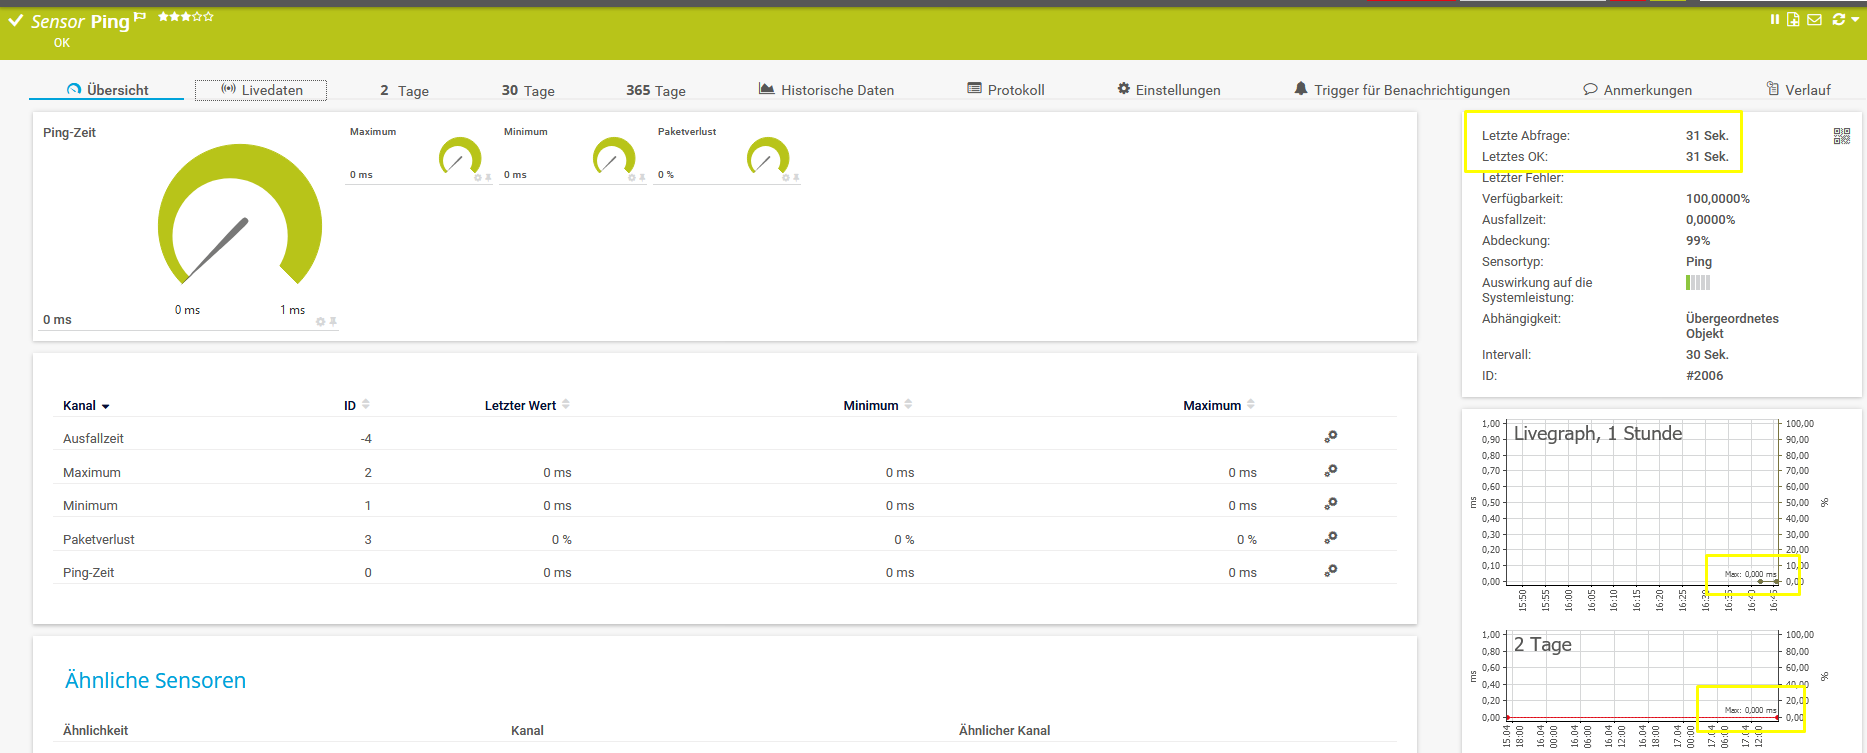
\includegraphics{./images/prtg_ping_statistik.png}
\caption{PRTG Sensor Statistiken}
\end{figure}

\hypertarget{apache-server-uxfcberwachen}{%
\subsubsection{Apache Server
überwachen}\label{apache-server-uxfcberwachen}}

Auf dem Linux Server wurde kurzerhand ein Apache Server installiert.
Über den HTTP Sensor lässt sich auch dieser ziemlich schnell und einfach
überwachen. Dazu dem selben Prozedere wie zuvor folgen.

\begin{figure}[!htb]
\centering
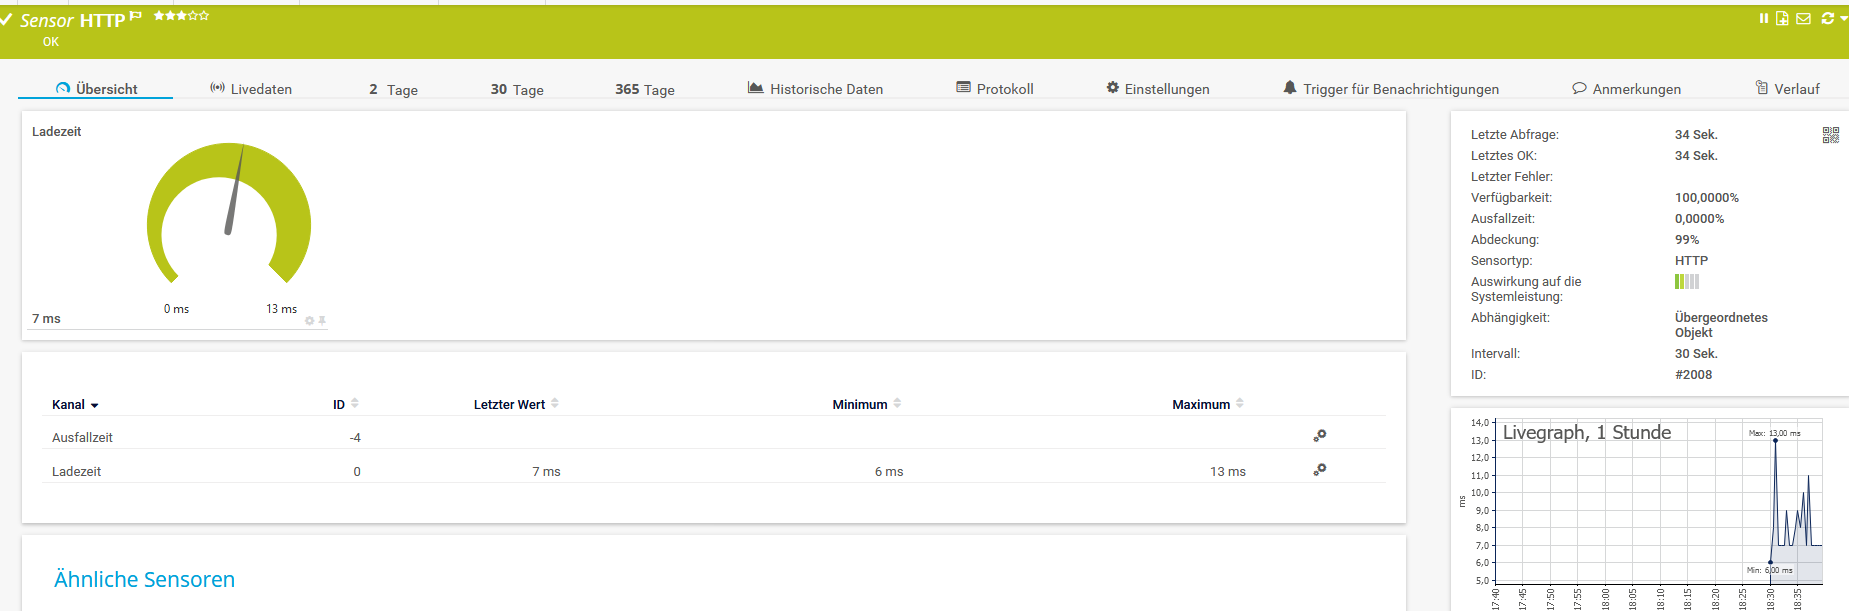
\includegraphics{./images/prtg_http.png}
\caption{PRTG Überwachung des Apache Serverss}
\end{figure}

Diesmal wollen wir allerdings eine Benachrichtigung erhalten, sobald der
Apache Server einen Fehler aufweist. Hierfür muss auf der Geräte Seite
unter dem Tab \emph{Trigger für Benachrichtigungen} ein neuer Trigger
hinzugefügt werden. In unserem Fall soll der Trigger nach 20 Sekunden
durchgehendem fehlerhaften Verhalten ein Ticket erstellt werden.

\begin{figure}[!htb]
\centering
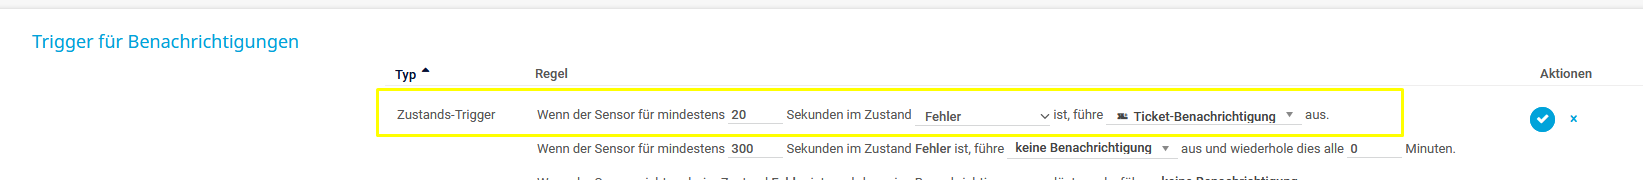
\includegraphics{./images/prtg_ticker.png}
\caption{PRTG Triggeraktion}
\end{figure}

Um zu testen wurde der Apache Server kurzerhand gestoppt und wie zu
erwarten wurde ein wenig später ein Ticket erstellt.

\begin{figure}[!htb]
\centering
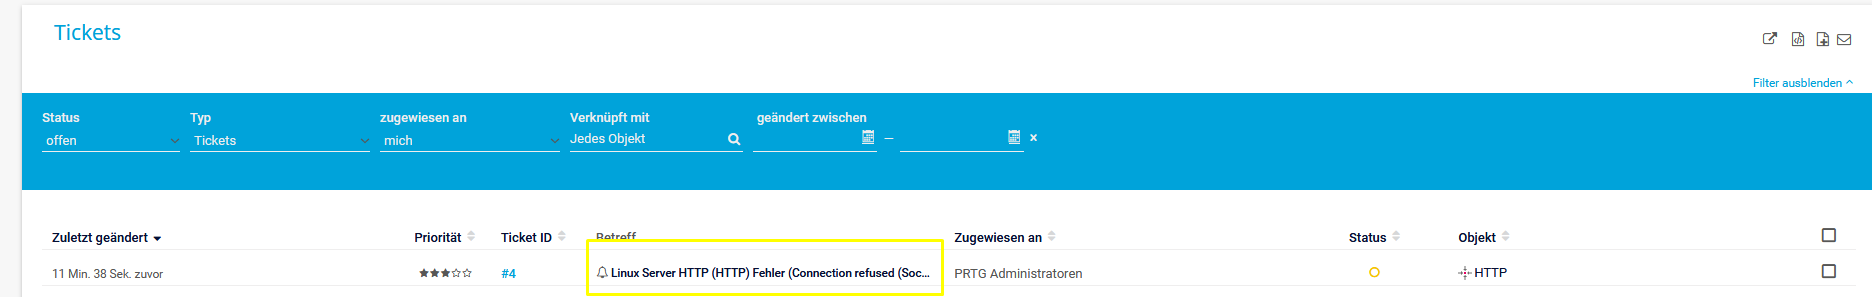
\includegraphics{./images/prtg-created-ticket.png}
\caption{PRTG Ticket}
\end{figure}

Mit einem Klick auf das Ticket können Details angezeigt werden
(Abbildung \ref{prtg-ticket}).

\begin{figure}[!htb]
\centering
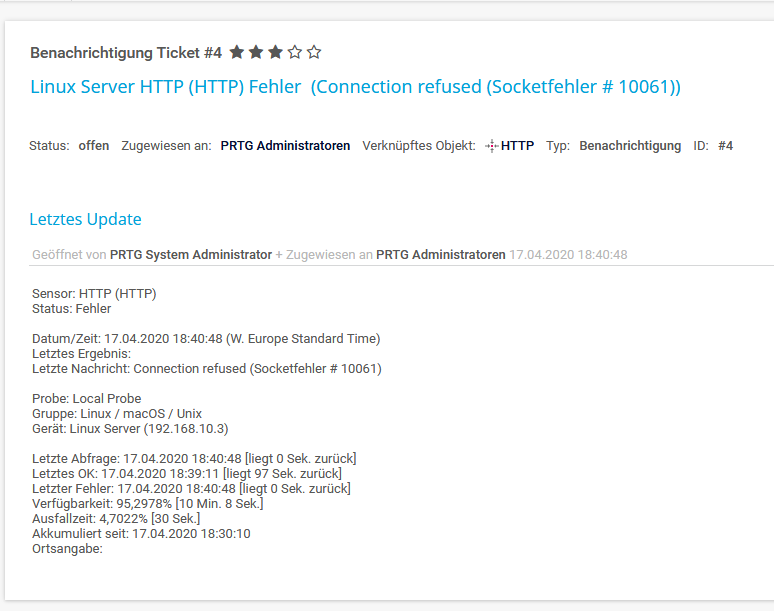
\includegraphics{./images/prtg-ticket-details.png}
\caption{PRTG Ticketdetails}\label{prtg-ticket}
\end{figure}

\hypertarget{erweiterte-sensoren}{%
\subsubsection{Erweiterte Sensoren}\label{erweiterte-sensoren}}

Um einen - meines Erachtens - recht außergewhönlichen Sensor zu
testen/implementieren. Wurde auf dem Linux Server mittels Flask und
Python eine REST-Api programmiert um den PRTG REST Sensor zu testen.

\begin{Shaded}
\begin{Highlighting}[]
\ImportTok{from}\NormalTok{ flask }\ImportTok{import}\NormalTok{ Flask, jsonify}

\NormalTok{app }\OperatorTok{=}\NormalTok{ Flask(}\VariableTok{\_\_name\_\_}\NormalTok{)}

\AttributeTok{@app.route}\NormalTok{(}\StringTok{"/"}\NormalTok{)}
\KeywordTok{def}\NormalTok{ hellOWorld():}
    \ControlFlowTok{return}\NormalTok{ jsonify(\{}\StringTok{"hallo"}\NormalTok{ : }\StringTok{"welt"}\NormalTok{\})}


\ControlFlowTok{if}\NormalTok{ \_\_name }\OperatorTok{==} \StringTok{\textquotesingle{}main\_\_\textquotesingle{}}\NormalTok{:}
\NormalTok{    app.run(host}\OperatorTok{=}\StringTok{\textquotesingle{}192.168.10.3\textquotesingle{}}\NormalTok{, port}\OperatorTok{=}\DecValTok{8080}\NormalTok{)}
\end{Highlighting}
\end{Shaded}

die mit REST API\(\footnote{noch in der BETA Version}\) Sensor überprüft
werden kann. Untr dem Reiter \emph{Historische Daten} kann man die
gesammelten Daten als CSV, kann man alle gesammelten Daten im CSV, XML
oder HTML exportieren um daraus z.B. Grafiken zu generieren. Zusätzlich
können Paremter wie der Zeitraum, das Durchschnittsinterval und die
gesammelten Kanäle angepasst werden.

\begin{figure}[!htb]
\centering
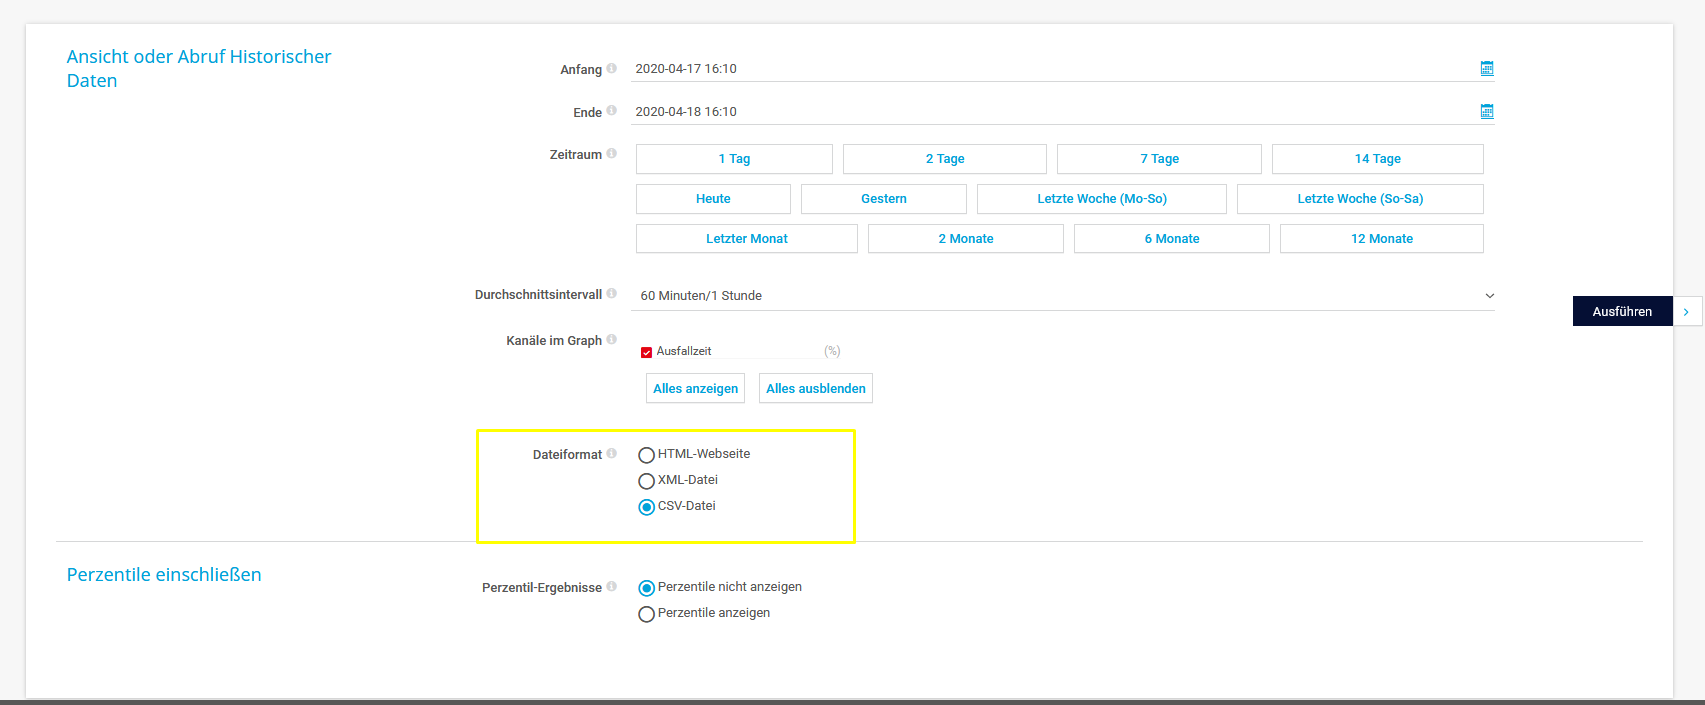
\includegraphics{./images/prtg-export.png}
\caption{PRTG Export von Daten}
\end{figure}

Mittels Excel können die Daten dann aufbereitet und weiterverarbeitet
werden, sofern man das möchte. Wir haben zur Veranschaulichung ein
Diagramm (Abbildung \ref{prtg-dia}) über die Performance der ReST-API
erstellt.

\begin{figure}[!htb]
\centering
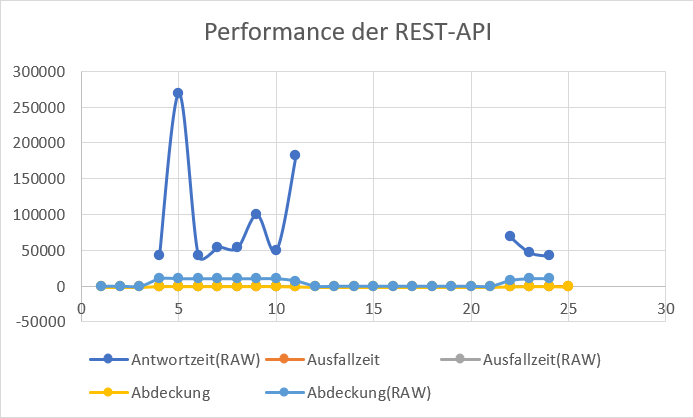
\includegraphics{./images/prtg-excel-stat.png}
\caption{PRTG REST-Performance Diagramm}\label{prtg-dia}
\end{figure}

Mit PRTG ist es auch möglich über eine SSH-Session, Informationen über
einen Server auszulesen wie z.B. die verfügbare Speicherauslastung.

\begin{figure}[!htb]
\centering
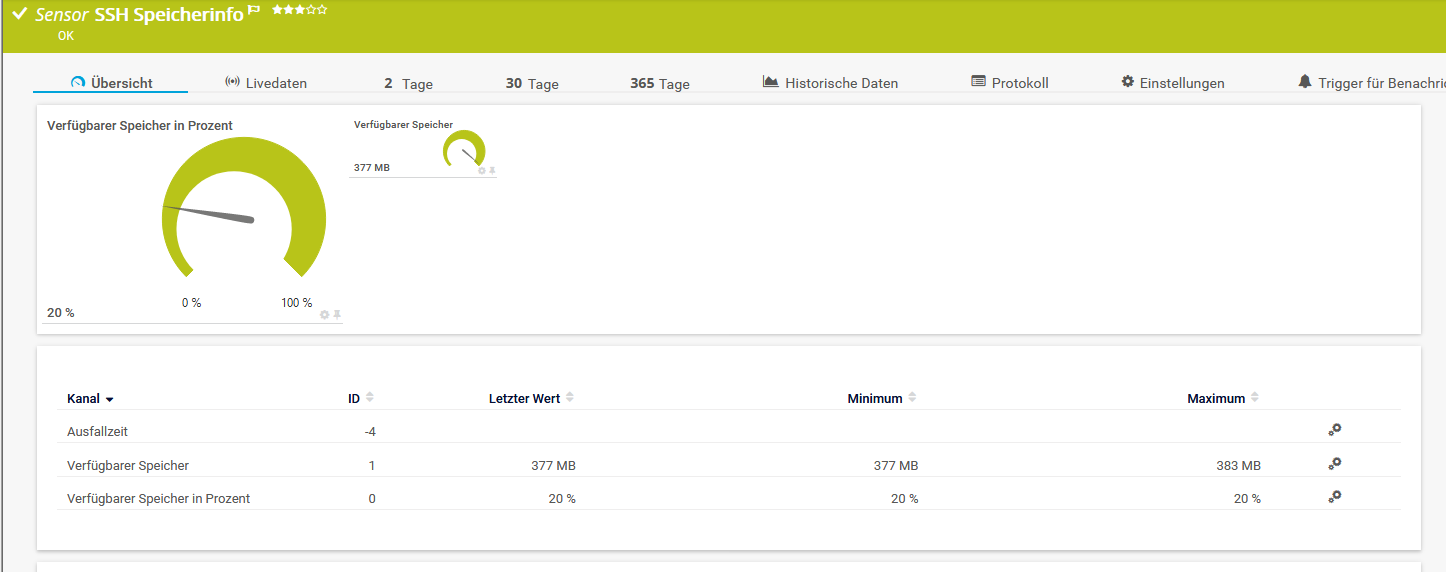
\includegraphics{./images/prtg-ssh-speicher.png}
\caption{PRTG SSH-Speicherauslastung}
\end{figure}

\hypertarget{uxfcberwachung-windows-server}{%
\subsection{Überwachung Windows
Server}\label{uxfcberwachung-windows-server}}

Die Überwachung eines Windows-Servers geht ein wenig anders von statten.
Hier findet der Informationsaustausch über
WMI\(\footnote{Windows Management Instrumentation}\), Performance
Counters oder SNMP statt. Die Vorteile bei SNMP liegen darin, dass es
eine deutlich geringere last verursacht, als seine Microsoftproprietären
Alternativen. Damit eht jedoch einher, dass WMI und Performance Counters
eine größere Menge an Daten anbieten, was bei einer rundum Überwachung
das um und auf ist.

In unserem Fall werden wir Log-Datein über de Windows Management
Instrumentations auswerten und einen modifizierten Sensor erstellen, der
bei dem Überschreiten eines Schewellenwertes ein Ticket erstellt.
Genauer der Ordner Desktop bei dem ab 4 Files ein neues Ticket erstellt
wird.

Im ersten Schritt muss der Sensor hinzugefügt werden. Dazu dem
vorherigen Prozedere folgen. Danach im Reiter \emph{Trigger für
Benachrichtigungen} ein neuer \emph{Schwellenwerttrigger} hinzugefügt
werden.

\begin{figure}[!htb]
\centering
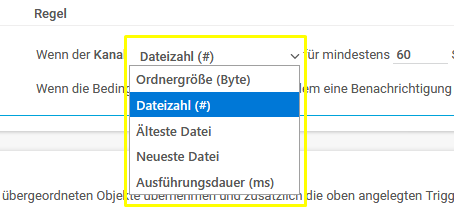
\includegraphics{./images/prtg_kanal.png}
\caption{PRTG Dateikanäle}
\end{figure}

Wenn man nun einige Dateien erstellt und ein wenig wartet erscheint
unter dem \emph{Tickets} Reiter ein neues Ticket:

\begin{figure}[!htb]
\centering
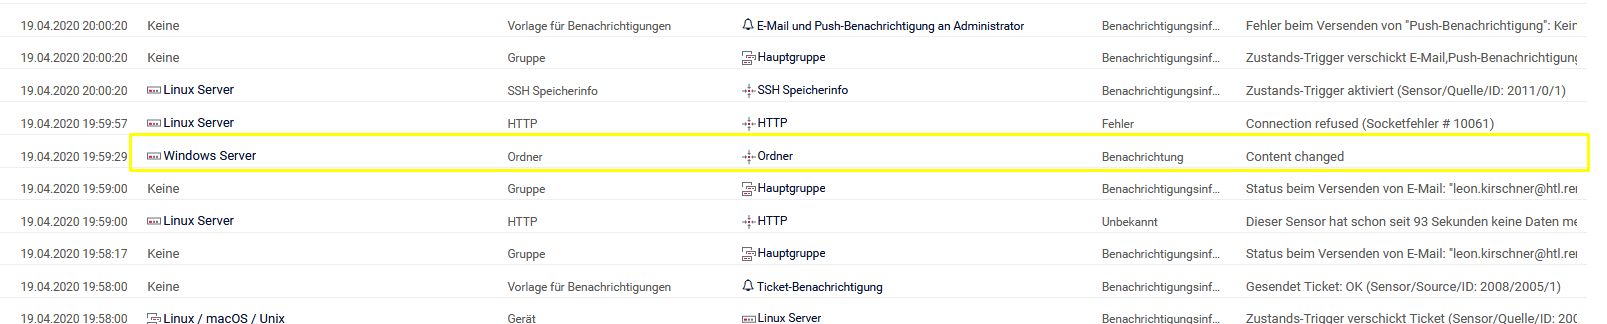
\includegraphics{./images/prtg-ticket-folder.png}
\caption{PRTG Schwellenwertfolder}
\end{figure}

\hypertarget{lessons-learned}{%
\section{Lessons Learned}\label{lessons-learned}}

Die Arbeit und das erkunden mit PRTG hat uns viel Spaß gemacht. Da
unsere VMs in der Schule zwei mal gelöscht wurden, ging jedoch leider
viel Zeit für die Windows- bzw. Linux Installation drauf, die wir gerne
in PRTG investiert hätten. Nichtsdestotrotz ist unser Fazit, dass PRTG
ein sehr mächtiges - wenn auch teures - Tool zur Überwachung eines
Netzwerkes ist. Der große Unterschied zu seinen (Open Source)
Konkurenten wie Nagios, wirbt es damit, keine Plugins anzubieten weil es
standardmäßig alles kann. Auch wenn wir nicht alles im Protokoll
vermerken konnten sind wir der Meinung, dass PRTG seinem Ruf gänzlich
gerecht wird. Durch das intuitive Web-UI ist es auch möglich, relativ
schnell und ohne viel Vorwissen Sensoren hinzuzufügen und ein IT-System
überwachen kann.
